\documentclass{sigchi}

% Use this command to override the default ACM copyright statement (e.g. for preprints). 
% Consult the conference website for the camera-ready copyright statement.
\toappear{
Second draft
% Submitted for review.
}

% Arabic page numbers for submission. 
% Remove this line to eliminate page numbers for the camera ready copy
\pagenumbering{arabic}


% Load basic packages
\usepackage{balance}  % to better equalize the last page
\usepackage{graphics} % for EPS, load graphicx instead
%%\usepackage{graphicx}
\usepackage{times}    % comment if you want LaTeX's default font
\usepackage{url}      % llt: nicely formatted URLs

% llt: Define a global style for URLs, rather that the default one
\makeatletter
\def\url@leostyle{%
  \@ifundefined{selectfont}{\def\UrlFont{\sf}}{\def\UrlFont{\small\bf\ttfamily}}}
\makeatother
\urlstyle{leo}


% To make various LaTeX processors do the right thing with page size.
\def\pprw{8.5in}
\def\pprh{11in}
\special{papersize=\pprw,\pprh}
\setlength{\paperwidth}{\pprw}
\setlength{\paperheight}{\pprh}
\setlength{\pdfpagewidth}{\pprw}
\setlength{\pdfpageheight}{\pprh}

% Make sure hyperref comes last of your loaded packages, 
% to give it a fighting chance of not being over-written, 
% since its job is to redefine many LaTeX commands.
\usepackage[pdftex]{hyperref}
\hypersetup{
pdftitle={User Modeling in Exploratory Search},
pdfauthor={LaTeX},
pdfkeywords={SIGCHI, proceedings, archival format},
bookmarksnumbered,
pdfstartview={FitH},
colorlinks,
citecolor=black,
filecolor=black,
linkcolor=black,
urlcolor=black,
breaklinks=true,
}

\DeclareGraphicsExtensions{.pdf,.png,.jpg}

% create a shortcut to typeset table headings
\newcommand\tabhead[1]{\small\textbf{#1}}


% End of preamble. Here it comes the document.
\begin{document}

\title{User Modeling in Exploratory Search}

\def\tktl{Department of Computer Science\\University of Helsinki}
\def\tktladdr{P.O. Box 68 (Gustaf H\"allstr\"omin katu 2b)\\
FI-00014 UNIVERSITY OF HELSINKI\\
FINLAND}

\numberofauthors{2}
\author{
  \alignauthor Ilkka Kiistala\\
    \affaddr{\tktl}\\
    % \affaddr{\tktladdr}\\
    \email{ilkka.kiistala@helsinki.fi}
  \alignauthor Tuire Peurala\\
    \affaddr{\tktl}\\
    % \affaddr{\tktladdr}\\
    \email{tuire.peurala@helsinki.fi}
}

\maketitle

\begin{abstract}
Here we'll describe the content of our essay.
\end{abstract}

\keywords{
Exploratory Search; Information Retrieval; User Modeling.
}

\category{H.5.m.}{Information Interfaces and Presentation (e.g. HCI)}{Miscellaneous}


\terms{
Human Factors; Design; Measurement. 
}

\section{Introduction}
Context – who needs, what needs, why that is a problem in current situation 

We'll describe here the roles of further chapters.

\section{User modeling}
\label{sec:usermodeling}
Shortish explanation of user modeling key concepts. 
\cite{rich99}, \cite{fischer01}

\subsection{Sterotypes}
Modeling stereotypes. 
% HCI reference needed
\cite{dillon96}, \cite{pu02}


\subsection{How to Collect and Analyze User Information}
% Pazzani puhuu "user profileista"
\cite{pazzani97}, \cite{white10}

\subsection{Personalization}
Individualization of user models, Adaptive/Adaptable User Interfaces, intelligent user interfaces
\cite{bunt04}, \cite{findlater04}, \cite{brusi96}

\cite{van08}: The writers are researchers at University of Twente, Netherlands. They took a look at scientific articles about “user-centered evaluation (UCE) studies of adaptive and adaptable systems”. The articles they reviewed are from 2007 and before. They reviewed 63 studies. Of the systems in the studies, 37 \% were adaptive, 27 \% adaptable and the rest, 36 \%, were both adaptive and adaptable. As a result of their literature review, they have modeled a process that can be used in evaluating a personalized system.
The model they present, “the iterative design process for a personalized system”, has four phases based on how ready the system is. Based on their findings in the studies they reviewed, they connect the most useful methods to use and most appropriate variables to investigate in each phase.
Overall, the article notes that “the current UCE practice of personalized systems was found to be sloppy at times”. They found that some of the questionnaires they reviewed were poorly designed and suggest that all the questionnaire data and log data as well should be made available so that a reader can judge the quality of the study. One reason they mention for low quality evaluations is that most evaluators of personalized systems are computer scientists and not specialized in evaluation.
\section {Exploratory search is a subtopic of information retrieval}

\subsection{Information retrieval}
There are many goals in information retrieval and exploratory search is one of them.
\cite{hearst02}, \cite{kuhlt91}

\cite{hearst06}: The article introduces two ways of grouping search results; clustering and hierarchical faceted categories. Clustering is grouping of items based on some similarity and is fully automated process. It is good for clarifying a vague query but the clustering algorithms aren't yet perfect and the clustering can be unpredicted. Category system is a set of labels that are organized to mirror the domain. Hierarchical faceted categories is a set of hierarchical categories that each represent a different dimension. Categories are usually created manually but can be partly automated. The article summarises good and bad parts of both grouping methods

\subsection{Exploratory Search}
Introduction to exploratory search.
\cite{march06}, \cite{white09}, \cite{tvaro11}

%% Palstan leveys tuntuu olevan n. 245pt

%\begin{figure}[p]
%\centering
%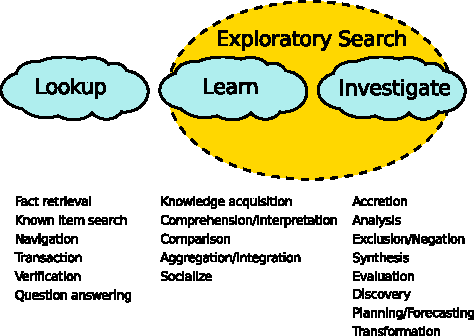
\includegraphics[bb=0 0 228 162]{clouds}
%\caption{Three clouds}
%\label{fig:clouds}
%\end{figure}

\section{User modeling in exploratory search}
Generally
\cite{oconnor10}, \cite{sugi04}, \cite{white07}, \cite{kules09}

\cite{kules09}:The writers had done a user experiment to find out what  the searchers are  looking at in a faceted search UI. The test participants were  university students and the system of interest was a library system. As a result  of the eyetracker test the writers found out that participants looked a lot at the facets and  47,4\% of the  eye movement  was between facets, breadcrums summarising the selected facets and the result list. In an interview the participants told they used facets to help organize their view on the topic domain and select sub-topics for further investigation. Of these results the researchers deduced that the facets played an important role in the exploratory search process. 
The article summarizes related study on faceted search and exploratory search and has many interesting leads on articles for our essay topic.
\subsection{User Model Construction Methods}

\subsection{Utilizing the User Model}

Search interface and search results, how they are affected by User Model?

Stereotypes used? Personalization used?

\subsection{Experience}

How has user modeling been used in supporting exploratory search, example cases? What challenges have emerged? 

- Cases

\subsection{Analysis}

- Challenges
- Success
- Failures

\subsection{Recommendations, Future improvement needs etc.}

See Cases: Conclusions

\section{Conclusion}
Goal, solution summary

Our goal was to explore the field of Exploratory Search and User Modeling. We found several articles that have some contribution to the topic.

Summary of results and their reliability 

We found that:
- Usage
- Success
- Failures

How much is it used in the real world, really?

Research impact
- What has the research brought into software development?

\nocite{*} %tämä listaa kaikki viitteet luetteloon vaikka niitä ei olisi vielä viitattu

% Balancing columns in a ref list is a bit of a pain because you
% either use a hack like flushend or balance, or manually insert
% a column break.  http://www.tex.ac.uk/cgi-bin/texfaq2html?label=balance
% multicols doesn't work because we're already in two-column mode,
% and flushend isn't awesome, so I choose balance.  See this
% for more info: http://cs.brown.edu/system/software/latex/doc/balance.pdf
%
% Note that in a perfect world balance wants to be in the first
% column of the last page.
%
% If balance doesn't work for you, you can remove that and
% hard-code a column break into the bbl file right before you
% submit:
%
% http://stackoverflow.com/questions/2149854/how-to-manually-equalize-columns-
% in-an-ieee-paper-if-using-bibtex
%
% Or, just remove \balance and give up on balancing the last page.
%
\balance

% If you want to use smaller typesetting for the reference list,
% uncomment the following line:
% \small
\bibliographystyle{acm-sigchi}
\bibliography{umines}
\end{document}
